Возьмем искусственный датасет с двумя признаками и одной зависимой переменной, чтобы испытать описанные методы. Выбрано именно два признака, чтобы была возможность визуально посмотреть на набор данных и увидеть закономерности в них, а также усложнить задачу алгоритмам, используя трехмерное пространство вместо двумерного.

Зависимая переменная задается следующей формулой:
\[
y = \frac{e^{-x^2-6x+5}}{70000} \cdot z - 3 \sin 0.3x + \sqrt{|x|} \cdot z^2
\]

График данной функции:

\vspace{-3mm}
\begin{figure}[h]
	\centering{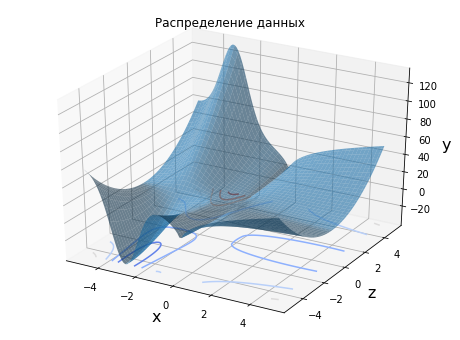
\includegraphics[width=0.6\linewidth]{pics/data.png}}
\end{figure}
\vspace{-3mm}

Переменные $x$ и $z$ сгенерированы как независимые нормальные случайные величины. Для задач был выбран стандартный градиентный бустинг реализации $\verb|sklearn|$\\ ($\verb|GradientBoostingRegressor|$). Гиперпараметры подобраны кросс-валидацией. Подробнее об обучении и кросс-валидации \href{https://github.com/elizacc/CW/blob/master/data%20%26%20code/Quality_check.ipynb}{здесь}.